\documentclass[aps,pra,twocolumn,superscriptaddress,longbibliography]{revtex4-2}

\usepackage{amsmath,amssymb,amsthm,graphicx,xcolor,bm,braket,dcolumn,booktabs}
\usepackage{hyperref}

\newtheorem{theorem}{Theorem}

%% ========================================================================
\title{The Level~4 Natural Geometry:\\
Two-Center Two-Electron Molecules\\
in Molecule-Frame Hyperspherical Coordinates}
\thanks{Paper 15 in the Geometric Vacuum series}

\author{J.~Loutey}
\affiliation{Independent Researcher, Kent, Washington}

\date{March 16, 2026}

%% ========================================================================
%% ABSTRACT
%% ========================================================================
\begin{document}
\begin{abstract}
The natural geometry hierarchy assigns each separable quantum system
a coordinate system in which Coulomb singularities become boundary
conditions and the Laplace--Beltrami operator discretizes on a sparse graph:
$S^3$ for hydrogen (Paper~7), prolate spheroidal for H$_2^+$ (Paper~11),
and hyperspherical for helium (Paper~13).
The two-center, two-electron molecule H$_2$ combines all five Coulomb
singularities and has resisted a single natural coordinate system.
We introduce \emph{molecule-frame hyperspherical coordinates}
$(R_e,\alpha,\theta_1,\theta_2,\Phi)$ parameterized by the
dimensionless ratio $\rho = R/(2R_e)$, where $R$ is the internuclear
distance and $R_e$ the electronic hyperradius.
The electron--electron cusp appears at $\alpha=\pi/4$, $\theta_{12}=0$,
independent of molecular geometry---a structural advantage over
prolate spheroidal coordinates, where it is a coordinate singularity.
The angular eigenvalue problem depends on $(R,R_e)$ only through $\rho$,
collapsing a two-dimensional parameter sweep to one dimension.
A coupled-channel expansion in body-frame partial waves
$(l_1,m_1,l_2,m_2)$ with $l_1+l_2$ even (gerade symmetry) and
$m_1+m_2=0$, solved with a variational two-dimensional
$(R_e,\alpha)$ solver that avoids the adiabatic approximation,
recovers 94.1\% of the exact dissociation energy $D_e$ at
$l_{\max}=4$ with $\sigma$ and $\pi$ channels (29~channels),
exceeding the 92.4\% achieved by prolate spheroidal CI with algebraic
Neumann integrals (Paper~12).
The framework extends naturally to heteronuclear diatomics: for
HeH$^+$ ($Z_A=2$, $Z_B=1$), a charge-center origin shift and removal
of the gerade constraint recover 93.1\% of the exact $D_e$ at
$l_{\max}=4$ with $\sigma{+}\pi$ channels (57~channels).
The solver has a double-adiabatic coupled-channel structure---nuclear
coordinates as outer slow variable, hyperradius as inner slow variable,
angular channels as fast variables---generalizing the single-adiabatic
expansion of Paper~13.
\end{abstract}

\maketitle

%% ========================================================================
%% I. INTRODUCTION
%% ========================================================================
\section{Introduction}
\label{sec:intro}

The natural geometry principle, articulated in Paper~13~\cite{paper13},
asserts that every separable quantum system possesses a natural
coordinate system in which Coulomb singularities become boundary
conditions rather than coordinate singularities, enabling sparse graph
discretization with no fitted parameters.
Three levels of this hierarchy have been established and validated:

\begin{description}
\item[Level~1] \emph{One-center, one-electron} (H).  Fock's 1935
  stereographic projection~\cite{fock1935} maps the hydrogen atom to the
  unit $S^3$, where the $1/r$ Coulomb singularity becomes the conformal
  factor of the projection.  The discrete graph Laplacian on $S^3$ is
  mathematically equivalent to the Schr\"odinger equation
  (Paper~7~\cite{paper7}; 18/18 symbolic proofs).
\item[Level~2] \emph{Two-center, one-electron} (H$_2^+$).  In prolate
  spheroidal coordinates $(\xi,\eta,\phi)$, the two nuclear Coulomb
  singularities $1/r_A + 1/r_B$ separate into independent equations.
  Paper~11~\cite{paper11} achieves 0.70\% error for H$_2^+$ with a
  sparse finite-difference lattice.
\item[Level~3] \emph{One-center, two-electron} (He).  Hyperspherical
  coordinates $(R_e,\alpha,\hat r_1,\hat r_2)$ resolve the
  electron--electron cusp $1/r_{12}$ as a boundary condition at
  $\alpha=\pi/4$, $\theta_{12}=0$.  Paper~13~\cite{paper13} achieves
  0.05\% error for He with a single-channel adiabatic lattice.
\end{description}

Level~4---the two-center, two-electron molecule H$_2$---is the first
system requiring \emph{simultaneous} resolution of nuclear ($1/r_{iA}$,
$1/r_{iB}$) and electron--electron ($1/r_{12}$) singularities.
Paper~12~\cite{paper12} demonstrated that prolate spheroidal CI with
algebraic Neumann $V_{ee}$ integrals saturates at 92.4\% of the exact
dissociation energy $D_e$.  The remaining 7.6\% gap was attributed to the
electron--electron cusp, which is a coordinate singularity in
$(\xi_1,\eta_1,\xi_2,\eta_2)$ space and cannot be captured by any
polynomial basis in those coordinates.

The present paper introduces the Level~4 natural geometry: molecule-frame
hyperspherical coordinates that resolve the $e$--$e$ cusp while retaining
the anisotropic nuclear field through a coupled partial-wave expansion.
We demonstrate that this approach recovers 94.1\% of $D_e$ at
$l_{\max}=4$ with $\sigma{+}\pi$ channels using a variational 2D solver,
exceeding Paper~12 and confirming the cusp-resolution advantage.

%% ========================================================================
%% II. COORDINATE SYSTEM
%% ========================================================================
\section{Molecule-Frame Hyperspherical Coordinates}
\label{sec:coords}

\subsection{Definition}

Consider two nuclei $A,B$ with charges $Z_A = Z_B = Z$ separated by
distance $R$ along the $z$-axis, placed at $z = \pm R/2$.  Two electrons
have positions $\bm{r}_1, \bm{r}_2$ measured from the molecular midpoint.
We define:
\begin{align}
  R_e &= \sqrt{r_1^2 + r_2^2}\,,
    \label{eq:Re} \\
  \alpha &= \arctan(r_2/r_1)\,,\quad \alpha\in[0,\pi/2]\,,
    \label{eq:alpha}
\end{align}
so that $r_1 = R_e\cos\alpha$, $r_2 = R_e\sin\alpha$.  Each electron's
direction in the body-fixed frame (z-axis along the internuclear axis) is
specified by polar angle $\theta_i \in [0,\pi]$ and azimuthal angle
$\phi_i$.  For $\Sigma$ states (total $M = m_1 + m_2 = 0$), only the
relative azimuth $\Phi = \phi_1 - \phi_2$ enters.

The full coordinate set for a $\Sigma$ state at fixed $R$ is
\begin{equation}
  (R_e, \alpha, \theta_1, \theta_2, \Phi)\,,
  \label{eq:coords}
\end{equation}
with the azimuthal center-of-mass $\phi_1 + \phi_2$ integrated out.

\subsection{The controlling parameter \texorpdfstring{$\rho$}{rho}}

The dimensionless ratio
\begin{equation}
  \rho \equiv \frac{R}{2R_e}
  \label{eq:rho}
\end{equation}
controls the transition between limiting geometries:
\begin{itemize}
  \item $\rho \to 0$ (united atom, $R_e \gg R$): Level~3 He-like
    with $Z_{\rm eff} = Z_A + Z_B$.
  \item $\rho \sim 1$ (molecular regime): full Level~4 coupling.
  \item $\rho \to \infty$ (separated atoms, $R_e \ll R$): two
    independent Level~1 atoms.
\end{itemize}

\subsection{Volume element}

The Jacobian of the transformation
$(r_1,r_2) \to (R_e,\alpha)$ gives
\begin{equation}
  dV = R_e^5 \cos^2\!\alpha\,\sin^2\!\alpha\;
       \sin\theta_1\,\sin\theta_2\;
       dR_e\,d\alpha\,d\theta_1\,d\theta_2\,d\Phi\,.
  \label{eq:volume}
\end{equation}
After extracting the wavefunction as
$\Psi = R_e^{-5/2}(\cos\alpha\,\sin\alpha)^{-1}
 F(R_e)\,\Phi_\nu(\alpha,\theta_1,\theta_2,\Phi)$,
the Jacobian centrifugal potential is $15/(8R_e^2)$, identical to the
He case (Paper~13, Eq.~12).

\subsection{Cusp location}

The electron--electron distance is
\begin{equation}
  r_{12}^2 = R_e^2(1 - \sin 2\alpha\,\cos\theta_{12})\,,
  \label{eq:r12}
\end{equation}
so $r_{12} = 0$ requires $\alpha = \pi/4$ and $\theta_{12} = 0$.
This locus is \emph{independent of} $\rho$ (and hence of $R$ and $R_e$).
The Kato cusp condition
$(\partial\Psi/\partial r_{12})_{r_{12}=0} = \tfrac{1}{2}\Psi|_{r_{12}=0}$
is therefore a fixed boundary condition on the angular eigenfunction,
unaffected by the molecular geometry.

This is the structural advantage of Level~4 coordinates: the cusp is
always a boundary condition, never a coordinate singularity, for
\emph{any} internuclear separation.

\begin{figure}
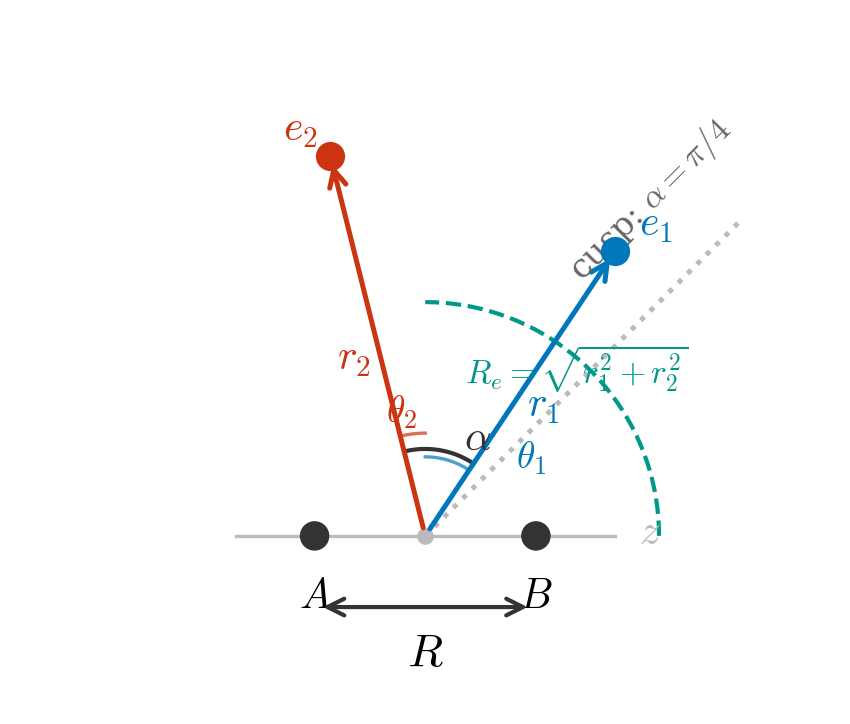
\includegraphics[width=\columnwidth]{paper_15_figures/level4_coordinates.png}
\caption{Molecule-frame hyperspherical coordinates for H$_2$.
  Two nuclei $A,B$ separated by $R$ define the body-frame $z$-axis.
  Electrons at $\bm{r}_1,\bm{r}_2$ from the midpoint are parameterized
  by hyperradius $R_e = \sqrt{r_1^2+r_2^2}$, correlation angle
  $\alpha = \arctan(r_2/r_1)$, and polar angles $\theta_1,\theta_2$
  from the internuclear axis.  The cusp locus $\alpha=\pi/4$ (dotted)
  is geometry-independent.}
\label{fig:coordinates}
\end{figure}

%% ========================================================================
%% III. THE MOLECULAR CHARGE FUNCTION
%% ========================================================================
\section{The Molecular Charge Function}
\label{sec:charge}

\subsection{Hamiltonian decomposition}

The electronic Hamiltonian at fixed $R$ decomposes in hyperspherical
coordinates as
\begin{equation}
  H_{\rm elec} = -\frac{1}{2}\frac{\partial^2}{\partial R_e^2}
    + \frac{\Lambda^2}{2R_e^2}
    + \frac{15}{8R_e^2}
    + V(R_e,\Omega;\rho)\,,
  \label{eq:Helec}
\end{equation}
where $\Lambda^2$ is the grand angular momentum on $S^5$ and the
potential is
\begin{equation}
  V = V_{\rm nuc} + V_{ee} + V_{NN}\,.
  \label{eq:Vtotal}
\end{equation}

\subsection{Electron--electron term}

The $e$--$e$ repulsion retains the He-like form:
\begin{equation}
  V_{ee} = \frac{1}{R_e}\,C_{ee}(\alpha,\theta_{12})\,,
  \label{eq:Vee}
\end{equation}
with
\begin{equation}
  C_{ee}(\alpha,\theta_{12}) =
    \frac{1}{\sqrt{1 - \sin 2\alpha\,\cos\theta_{12}}}\,.
  \label{eq:Cee}
\end{equation}
This charge function is $\rho$-independent: the $e$--$e$ interaction
depends only on the angular coordinates.

\subsection{Nuclear attraction}

The nuclear potential introduces $\rho$-dependence.  For electron $i$
at distance $r_i = R_e s_i$ from the midpoint (where $s_1 = \cos\alpha$,
$s_2 = \sin\alpha$):
\begin{equation}
  -\frac{Z}{r_{iA}} = -\frac{Z}{R_e}\,
    \frac{1}{s_i\sqrt{1 + (\rho/s_i)^2 + 2(\rho/s_i)\cos\theta_i}}\,,
  \label{eq:VnucA}
\end{equation}
with an analogous expression for nucleus $B$ ($\cos\theta_i \to
-\cos\theta_i$).  The full nuclear potential is
\begin{equation}
  V_{\rm nuc} = \frac{R_e}{R_e}\sum_{i=1}^2
    \bigl(-Z/r_{iA} - Z/r_{iB}\bigr)
  = \frac{1}{R_e}\,C_{\rm nuc}(\alpha,\theta_1,\theta_2;\rho)\,,
  \label{eq:Vnuc}
\end{equation}
but $C_{\rm nuc}$ depends on $\rho$ through Eq.~\eqref{eq:VnucA},
preventing a clean separation of $R_e$ and angular coordinates.

\subsection{The molecular charge function}

Combining Eqs.~\eqref{eq:Vee} and~\eqref{eq:Vnuc}:
\begin{equation}
  C_{\rm mol}(\alpha,\theta_1,\theta_2,\Phi;\rho)
    = C_{ee}(\alpha,\theta_{12})
    + C_{\rm nuc}(\alpha,\theta_1,\theta_2;\rho)\,.
  \label{eq:Cmol}
\end{equation}

In He ($\rho=0$), the nuclear term reduces to
$C_{\rm nuc} = -Z_{\rm tot}(1/\cos\alpha + 1/\sin\alpha)$
and becomes angular-only.  For $\rho > 0$, the $\theta_i$-dependence
of $C_{\rm nuc}$ mixes body-frame partial waves---the source of
inter-channel coupling in the multichannel expansion.

%% ========================================================================
%% IV. ADIABATIC SEPARATION
%% ========================================================================
\section{Double Adiabatic Approximation}
\label{sec:adiabatic}

\subsection{Two-stage Born--Oppenheimer}

The Level~4 problem has a natural double-adiabatic structure:
\begin{enumerate}
  \item \textbf{Outer (nuclear):} Fix $R$; solve for the electronic
    energy $E_{\rm elec}(R)$.
  \item \textbf{Inner (electronic):} At fixed $R$, decompose the
    electronic problem into a hyperradial coordinate $R_e$ (slow) and
    angular coordinates $\Omega = (\alpha,\theta_1,\theta_2,\Phi)$ (fast).
\end{enumerate}

\subsection{Angular eigenvalue problem}

At fixed $R_e$ (and hence fixed $\rho = R/(2R_e)$), the angular
eigenvalue problem is
\begin{equation}
  \Bigl[\tfrac{1}{2}\Lambda^2
    + R_e\,C_{\rm mol}(\Omega;\rho)\Bigr]
  \Phi_\nu(\Omega;R_e)
  = \mu_\nu(R_e)\,\Phi_\nu(\Omega;R_e)\,.
  \label{eq:angular}
\end{equation}

The key simplification: since $C_{\rm mol}$ depends on $(R,R_e)$
only through $\rho = R/(2R_e)$, the angular eigenstates and eigenvalues
at different $(R,R_e)$ pairs sharing the same $\rho$ are related by a
simple $R_e$-rescaling.  This collapses the \emph{a priori}
two-dimensional $(R,R_e)$ sweep to a one-dimensional $\rho$-sweep,
with substantial computational savings.

\subsection{Liouville substitution}

For the $l_1 = l_2 = 0$ channel, the Liouville substitution
$u(\alpha) = \sin\alpha\,\cos\alpha\;\phi(\alpha)$ transforms
the weighted Sturm--Liouville equation into standard Schr\"odinger form:
\begin{equation}
  -\tfrac{1}{2}u'' + V_{\rm eff}(\alpha;\rho)\,u = \mu\,u\,,
  \label{eq:liouville}
\end{equation}
with Dirichlet boundary conditions $u(0) = u(\pi/2) = 0$.  The
effective potential is
\begin{equation}
  V_{\rm eff}(\alpha) = -2
    + \frac{l_1(l_1+1)}{2\cos^2\!\alpha}
    + \frac{l_2(l_2+1)}{2\sin^2\!\alpha}
    + R_e\,C_{\rm mol}^{l_1 l_2}(\alpha;\rho)\,,
  \label{eq:Veff_alpha}
\end{equation}
where $C_{\rm mol}^{l_1 l_2}$ is the projection of $C_{\rm mol}$ onto
the $(l_1,l_2)$ channel (Sec.~\ref{sec:multichannel}).

\subsection{Hyperradial equation}

Given $\mu_\nu(R_e;R)$, the hyperradial equation is
\begin{equation}
  -\frac{1}{2}\frac{d^2 F_\nu}{dR_e^2}
  + \biggl[\frac{\mu_\nu(R_e;R) + 15/8}{R_e^2}\biggr]F_\nu
  = E_{\rm elec}\,F_\nu\,,
  \label{eq:radial}
\end{equation}
structurally identical to Paper~13, Eq.~18.  The adiabatic potential
$U(R_e;R) = [\mu(R_e;R) + 15/8]/R_e^2$ is computed by sweeping $R_e$
and solving Eq.~\eqref{eq:angular} at each point.

\subsection{Limiting cases}

\paragraph{United atom ($R\to 0$).}
As $\rho \to 0$, the nuclear term reduces to
$C_{\rm nuc} \to -(Z_A+Z_B)(1/\cos\alpha + 1/\sin\alpha)$,
recovering the He charge function with $Z = Z_A + Z_B$.
The angular equation~\eqref{eq:angular} becomes the Paper~13 equation
exactly.  Numerically verified: the Level~4 eigenvalue at
$\rho = 10^{-6}$ matches the He eigenvalue to machine precision.

\paragraph{One-electron limit.}
Removing electron~2 ($\alpha \to 0$, $r_2 \to 0$, $r_1 \to R_e$)
reduces the electronic problem to the one-electron H$_2^+$ Hamiltonian
in body-frame coordinates.  The angular eigenvalue problem becomes the
$\eta$-equation of prolate spheroidal coordinates (Paper~11).

%% ========================================================================
%% V. MULTICHANNEL EXPANSION
%% ========================================================================
\section{Multichannel Partial-Wave Expansion}
\label{sec:multichannel}

\subsection{Channel labels}

For $^1\Sigma_g^+$ symmetry with total $M = m_1 + m_2 = 0$, each
electron's angular part is expanded in spherical harmonics
$Y_{l_i}^{m_i}(\theta_i,\phi_i)$.  Channels are labeled by
4-tuples $(l_1,m_1,l_2,m_2)$.  Gerade symmetry under inversion requires
\begin{equation}
  l_1 + l_2 = \text{even}\,,
  \label{eq:gerade}
\end{equation}
and the constraint $m_1 + m_2 = 0$ enforces $\Sigma$ symmetry.
Both orderings $(l_1,l_2)$ and $(l_2,l_1)$ with $l_1 \ne l_2$ are
included as separate channels because they have distinct centrifugal
potentials: $l_1(l_1+1)/\cos^2\!\alpha$ vs.\ $l_2(l_2+1)/\cos^2\!\alpha$.

\paragraph{$\sigma$ and $\pi$ channels.}
Channels with $m_1 = m_2 = 0$ are $\sigma$~channels; the angular
expansion uses Legendre polynomials $P_{l_i}(\cos\theta_i)$ and
depends only on $\theta_1,\theta_2$ (no $\Phi$-dependence).
Channels with $|m_i| \ge 1$ are $\pi,\delta,\ldots$~channels;
they introduce $\Phi$-dependence through the associated Legendre
functions and couple to $\sigma$~channels via the $e$--$e$ multipole
expansion.  The nuclear potential is diagonal in $m$ (axial symmetry),
so $\sigma$--$\pi$ coupling arises exclusively from $V_{ee}$.

The channel count for $l_{\max}$ is $(l_{\max}+1)^2/2$ (approximately):

\begin{center}
\begin{tabular}{ccl}
\toprule
$l_{\max}$ & $N_{\rm ch}$ & Channels \\
\midrule
0 & 1 & (0,0) \\
1 & 2 & (0,0), (1,1) \\
2 & 5 & (0,0), (0,2), (2,0), (1,1), (2,2) \\
3 & 8 & $+$ (1,3), (3,1), (3,3) \\
4 & 13 & $+$ (0,4), (4,0), (2,4), (4,2), (4,4) \\
\bottomrule
\end{tabular}
\end{center}

\subsection{Electron--electron coupling}

The multipole expansion of $1/r_{12}$ in the body-frame basis gives
\begin{equation}
  \braket{l_1' l_2' | C_{ee} | l_1 l_2}
  = \mathcal{N}\!\sum_k
    G(l_1',k,l_1)\,G(l_2',k,l_2)\,\frac{f_k(\alpha)}{\max(s_1,s_2)}\,,
  \label{eq:Wee}
\end{equation}
where $G(l,k,l')$ is the Gaunt integral
$\int_{-1}^1 P_l\,P_k\,P_{l'}\,dx$, the function
$f_k(\alpha) = [\min(\cos\alpha,\sin\alpha)/\max(\cos\alpha,\sin\alpha)]^k$,
and the normalization is
$\mathcal{N} = \sqrt{(2l_1'+1)(2l_2'+1)(2l_1+1)(2l_2+1)}/4$.

The selection rules on Gaunt integrals enforce sparsity:
$G(l,k,l') = 0$ unless $l+k+l'$ is even and $|l-l'| \le k \le l+l'$.
In the product of two Gaunt integrals, $k$ must simultaneously
satisfy conditions from both factors.

\subsection{Nuclear coupling}

The nuclear attraction couples channels because it depends on
$\theta_i$:
\begin{multline}
  \braket{l_1' l_2' | C_{\rm nuc} | l_1 l_2}
  = N_1\!\int_{-1}^1\! P_{l_1'}\,V_1(x;\alpha,\rho)\,P_{l_1}\,dx\;\delta_{l_2' l_2}
  \\
  + \delta_{l_1' l_1}\,N_2\!\int_{-1}^1\! P_{l_2'}\,V_2(x;\alpha,\rho)\,P_{l_2}\,dx\,,
  \label{eq:Wnuc}
\end{multline}
where $V_i(x;\alpha,\rho) = -Z/d_{iA} - Z/d_{iB}$ with
$d_{iA} = \sqrt{s_i^2 + \rho^2 + 2\rho s_i x}$, and
$N_j = \sqrt{(2l_j'+1)(2l_j+1)}$ ensures consistency with the
orthonormal $\hat P$ basis.

A single Legendre expansion of $V_i$ in powers of $\rho/s_i$
diverges when $\rho/s_i > 1$ (electron between midpoint and
nucleus).  We resolve this by splitting into two convergent regions:
for $\rho < s_i$, expand in $(\rho/s_i)^k$; for $\rho > s_i$,
expand in $(s_i/\rho)^k$.  In each region, the $\theta$-integral
reduces to a sum over Gaunt integrals
\begin{equation}
  G(l', k, l) = 2\begin{pmatrix} l' & k & l \\ 0 & 0 & 0
  \end{pmatrix}^{\!2},
  \label{eq:gaunt_nuc}
\end{equation}
proportional to the square of a Wigner $3j$ symbol---the same
objects that appear in the electron--electron coupling
(Paper~13~\cite{paper13}, Sec.~III.C).
The triangle inequality $|l' - l| \leq k \leq l' + l$ forces
the sum to terminate exactly at $k = l' + l$: no truncation
parameter is needed.  The result is exact to machine precision
in all regimes, including the boundary $\rho/s_i = 1$ where
the two expansions match continuously.

Gauss--Legendre quadrature is used only in the screened
($Z_{\rm eff}$) path for composed geometries (Paper~17), where
the smooth correction $[Z_A - Z_{\rm eff}(r)]/r$ is
non-polynomial and the algebraic expansion does not apply.

\paragraph{Critical observation.}
The nuclear coupling requires \emph{one} $l$-index to match via the
Kronecker delta while the other index transitions via the integral.
Thus the (0,0) channel couples to (0,2) through electron~2 and to
(2,0) through electron~1.  Omitting either ordering halves the
nuclear coupling strength.

\subsection{The gerade--quadrupole constraint}

The gerade constraint $l_1 + l_2 = \text{even}$ forces the first
nuclear coupling from (0,0) to involve $\Delta l = 2$ transitions:
\begin{equation}
  (0,0) \longrightarrow (0,2),\;(2,0)\qquad(\text{quadrupolar})\,.
  \label{eq:quadrupole}
\end{equation}
Dipolar transitions ($\Delta l = 1$) would couple to (0,1) or (1,0),
but $l_1 + l_2 = 1$ is odd and excluded.  This explains why $l_{\max}=1$
barely improves on $l_{\max}=0$: the (1,1) channel has no nuclear
coupling to (0,0) (both Kronecker deltas are zero) and only weak
$e$--$e$ coupling.

The jump at $l_{\max} = 2$ (31\% $\to$ 88\%) reflects the onset of
nuclear coupling.

\subsection{Heteronuclear extension}
\label{sec:heteronuclear}

For heteronuclear diatomics ($Z_A \ne Z_B$), three modifications are
required:

\paragraph{1.\ Removal of the gerade constraint.}
The gerade symmetry $l_1 + l_2 = \text{even}$ relies on the
inversion symmetry $\theta_i \to \pi - \theta_i$ exchanging
identical nuclei.  When $Z_A \ne Z_B$, this symmetry is absent
and the channel list includes all $(l_1, l_2)$ pairs with
$l_1, l_2 \le l_{\max}$.  At $l_{\max} = 4$, $m_{\max} = 0$,
this doubles the channel count from 13 (homonuclear) to 25
(heteronuclear).

\paragraph{2.\ Odd-$k$ nuclear multipole coupling.}
The nuclear potential becomes
\begin{equation}
  V_{\rm nuc}^{(i)} = -\sum_{k=0}^{\infty}
    \Bigl[Z_A\,f_k(s_i,\rho_A)
    + Z_B\,(-1)^k\,f_k(s_i,\rho_B)\Bigr]\,P_k(\cos\theta_i)\,,
  \label{eq:Vnuc_hetero}
\end{equation}
where the $(-1)^k$ factor encodes the opposite-pole geometry.
For homonuclear systems ($Z_A = Z_B$), the odd-$k$ coefficient
$Z_A - Z_B = 0$ and only even-$k$ terms survive.  For
heteronuclear systems, odd-$k$ terms (dipole, octupole, \ldots)
contribute with strength proportional to $Z_A - Z_B$.
The $k$-parity of each coupling matrix element is fixed by
the 3-$j$ symbol: $\bigl(\begin{smallmatrix} l' & k & l \\
0 & 0 & 0 \end{smallmatrix}\bigr)$ requires $l' + k + l$ even,
so $k$ has the same parity as $l' + l$.

\paragraph{3.\ Charge-center origin.}
The coordinate origin is shifted from the geometric midpoint
toward the heavier nucleus:
\begin{equation}
  z_0 = \frac{R\,(Z_A - Z_B)}{2\,(Z_A + Z_B)}\,,
  \label{eq:charge_center}
\end{equation}
giving nuclear distances $R_A = R/2 - z_0$, $R_B = R/2 + z_0$,
and dimensionless ratios $\rho_A = R_A / R_e$,
$\rho_B = R_B / R_e$.  For $Z_A = Z_B$, $z_0 = 0$ and the
standard midpoint origin is recovered.  The charge-center origin
places the heavier nucleus closer to the coordinate center,
improving the convergence of the partial-wave expansion by
approximately one unit of $l_{\max}$.

\paragraph{Channel weight distribution.}
The ground-state angular eigenfunction distributes weight across
channels as follows: for H$_2$ at $\rho = 0.7$, 77\% of the norm
resides in the $(0{,}0)$ channel and 3~channels suffice for 90\%.
For a $6{:}1$ charge ratio (modeling O--H bonds), only 26\% resides
in $(0{,}0)$ and 8~channels are needed for 90\%.  The dipolar
channels $(0{,}1) + (1{,}0)$ carry 36\% of the norm---more than
$(0{,}0)$ itself---reflecting the strong $P_1(\cos\theta)$ component
of the asymmetric nuclear potential.  This spreading is entirely
from the nuclear coupling; the electron--electron interaction
contributes no off-diagonal channel mixing ($w(0{,}0) = 0.9998$ with
$e$--$e$ coupling only).  The practical implication is that
asymmetric bonds require $l_{\max} \ge 4$ for qualitative accuracy,
compared to $l_{\max} = 2$ for homonuclear systems.

\paragraph{Dissociation limit.}
For heteronuclear two-electron systems, both electrons bind to the
larger-$Z$ nucleus at dissociation.  For HeH$^+$
($Z_A = 2$, $Z_B = 1$): $\text{HeH}^+ \to \text{He} + \text{H}^+$,
so $E_{\rm atoms} = E(\text{He}) = -2.9037$~Ha (exact
nonrelativistic).

%% ========================================================================
%% VI. RESULTS
%% ========================================================================
\section{Results}
\label{sec:results}

\subsection{Convergence with \texorpdfstring{$l_{\max}$}{l\_max}}

Table~\ref{tab:convergence} shows the convergence of
$D_e = 2E(\text{H}) - E_{\rm total}$ at $R = 1.4$~bohr, computed
with the variational 2D solver (Sec.~\ref{sec:2d_solver}).
The adiabatic approximation results are shown for comparison; the
${\sim}11\%$ gap between adiabatic and 2D results reflects the
non-adiabatic kinetic energy cost ignored by the adiabatic solver.

\begin{table}[h]
\caption{Convergence with partial-wave truncation.
  $\sigma$~channels have $m=0$ only; $\sigma{+}\pi$ includes
  $|m| \le 1$.  The 2D solver is variational; the adiabatic solver
  systematically overestimates $D_e$ by ${\sim}11\%$.
  $D_e^{\rm exact} = 0.17447$~Ha~\cite{kolos1968}.}
\label{tab:convergence}
\begin{ruledtabular}
\begin{tabular}{ccdddd}
$l_{\max}$ & $m_{\max}$ & \multicolumn{1}{c}{$N_{\rm ch}$}
  & \multicolumn{1}{c}{2D (\%)}
  & \multicolumn{1}{c}{Adiab.\ (\%)}
  & \multicolumn{1}{c}{Gap (\%)} \\
\hline
2 & 0 &  5 & 79.5 & 90.3 & 10.8 \\
2 & 1 &  9 & 86.2 & 96.8 & 10.6 \\
3 & 0 &  8 & 80.2 & 91.0 & 10.9 \\
3 & 1 & 18 & 87.1 & 97.7 & 10.7 \\
4 & 0 & 13 & 87.0 & 98.6 & 11.5 \\
4 & 1 & 29 & 94.1 & 105.2^* & 11.1 \\
\end{tabular}
\end{ruledtabular}
{\footnotesize ${}^*$Adiabatic variational violation; the 2D result
is the correct variational bound.}
\end{table}

\subsection{Comparison with Paper~12}

\begin{table}[h]
\caption{Comparison of Level~4 with Paper~12 prolate spheroidal CI
  (Neumann $V_{ee}$) and exact results.  All at $R = 1.4$~bohr.
  Level~4 results use the variational 2D solver.}
\label{tab:comparison}
\begin{ruledtabular}
\begin{tabular}{ldd}
Method
  & \multicolumn{1}{c}{$D_e$ (Ha)}
  & \multicolumn{1}{c}{$D_e/D_e^{\rm exact}$ (\%)} \\
\hline
Paper~12 (Neumann $V_{ee}$)                  & 0.1612 & 92.4 \\
Level~4 ($l_{\max}=4$, $\sigma$ only, 13~ch) & 0.1518 & 87.0 \\
Level~4 ($l_{\max}=4$, $\sigma{+}\pi$, 29~ch)& 0.1642 & 94.1 \\
Exact~\cite{kolos1968}                       & 0.1745 & 100.0 \\
\end{tabular}
\end{ruledtabular}
\end{table}

The $\sigma$-only result (87.0\%) falls below Paper~12, but adding
$\pi$~channels pushes the Level~4 result to 94.1\%---a
1.7~percentage-point improvement over Paper~12.  This confirms that
the hyperspherical coordinates' cusp resolution provides a genuine
advantage, but only when the angular basis includes both $\sigma$ and
$\pi$ partial waves.

\subsection{Grid convergence}

At fixed $l_{\max} = 3$, increasing $n_\alpha$ from 100 to 250 and
$n_{\rm quad}$ from 24 to 40 yields only a 1.3~percentage-point
improvement (88.5\% $\to$ 89.8\%), confirming that the partial-wave
truncation---not the finite-difference resolution---is the limiting
factor.

\begin{figure}
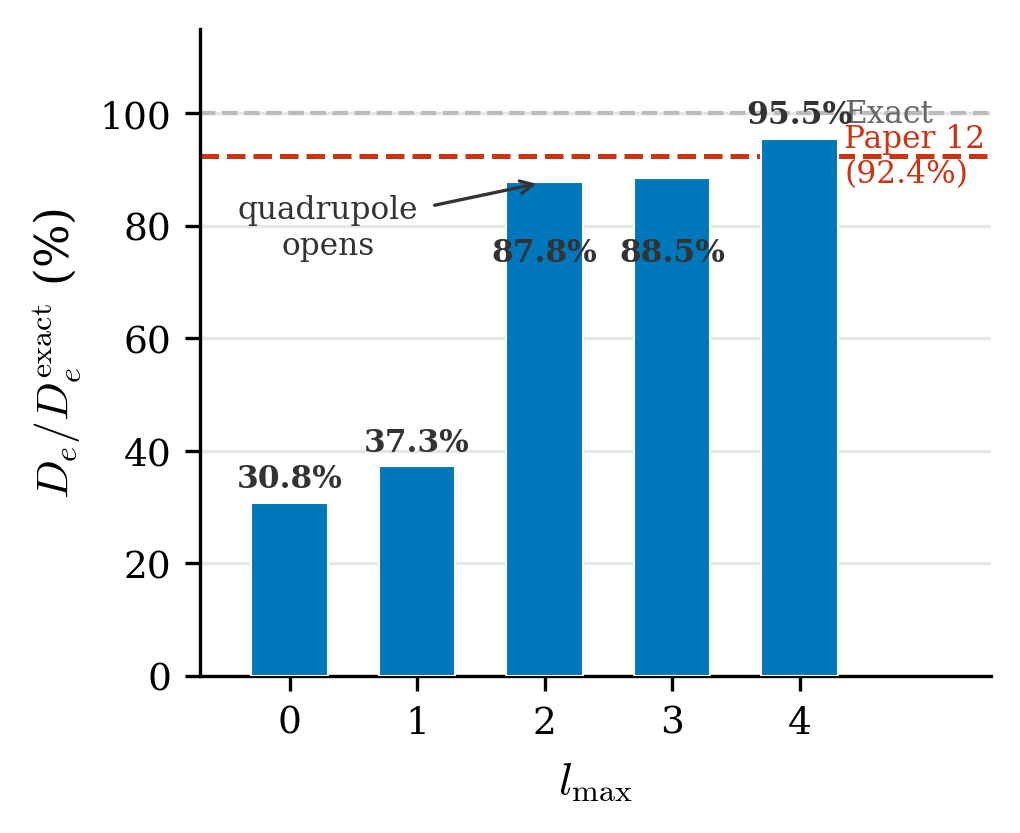
\includegraphics[width=\columnwidth]{paper_15_figures/convergence_lmax.png}
\caption{Percentage of exact dissociation energy recovered as a function
  of $l_{\max}$.  The dashed line marks Paper~12's 92.4\%.  The dramatic
  jump at $l_{\max}=2$ reflects the onset of quadrupolar nuclear
  coupling (Sec.~\ref{sec:multichannel}).}
\label{fig:convergence}
\end{figure}

\subsection{Variational 2D solver}
\label{sec:2d_solver}

The adiabatic approximation (Eq.~\ref{eq:radial}) neglects kinetic
coupling between angular channels as $R_e$ varies.  To obtain
rigorous variational bounds, we solve the full two-dimensional
$(R_e,\alpha)$ problem directly, building the sparse Hamiltonian
\begin{equation}
  H_{\rm 2D} = T_{R_e} \otimes I_{\rm ang}
    + \bigl[H_{\rm ang}(R_e) + \tfrac{15}{8}I\bigr] / R_e^2
  \label{eq:H2d}
\end{equation}
in the product space of $R_e$ grid $\times$ angular channels $\times$
$\alpha$ grid, and finding the lowest eigenvalue via shift-invert
Lanczos~\cite{lin1995}.  The matrix dimension is
$N_{R_e} \times N_{\rm ch} \times n_\alpha$; for $l_{\max}=4$,
$m_{\max}=1$ (29~channels, $n_\alpha = 60$, $N_{R_e} = 120$),
the sparse matrix has $N = 208{,}800$ rows and ${\sim}6.6 \times 10^6$
nonzeros, solved in ${\sim}2$~minutes.

The 2D solver consistently gives $D_e$ approximately 11\% lower
than the adiabatic solver (Table~\ref{tab:convergence}), confirming
that the adiabatic approximation systematically overestimates binding
by neglecting the kinetic energy cost of angular wavefunction
variation with $R_e$.

\subsection{HeH\texorpdfstring{$^+$}{+} convergence}
\label{sec:heh_results}

Table~\ref{tab:heh_convergence} shows convergence for
HeH$^+$ ($Z_A = 2$, $Z_B = 1$) at $R = 1.46$~bohr,
using the charge-center origin
($z_0 = R/6 = 0.243$~bohr; Eq.~\ref{eq:charge_center}).
The exact total energy is $-2.9787$~Ha and the exact
dissociation energy is $D_e = 0.0750$~Ha~\cite{bishop1977},
measured relative to the He ground state
($E_{\rm atoms} = -2.9037$~Ha).

\begin{table}[h]
\caption{HeH$^+$ convergence at $R = 1.46$~bohr with
charge-center origin.  $N_{\rm ch}$ is the number of channels.
The adiabatic solver is used for all entries.}
\label{tab:heh_convergence}
\begin{ruledtabular}
\begin{tabular}{ccccc}
$l_{\max}$ & $m_{\max}$ & $N_{\rm ch}$ &
  $E_{\rm total}$ (Ha) & $D_e / D_e^{\rm exact}$ \\
\hline
2 & 0 &  9 & $-2.764$ & unbound \\
3 & 0 & 16 & $-2.860$ & unbound \\
4 & 0 & 25 & $-2.961$ & 76.8\% \\
4 & 1 & 57 & $-2.974$ & 93.1\% \\
\end{tabular}
\end{ruledtabular}
\end{table}

The system is unbound at $l_{\max} \le 3$ ($\sigma$-only) because
the total energy lies above the He dissociation limit.  At
$l_{\max} = 4$ with $\sigma$-only channels, 76.8\% of $D_e$
is recovered; adding $\pi$ channels brings this to 93.1\%,
a 16-percentage-point improvement that mirrors the H$_2$ pattern.

The slower convergence compared to H$_2$ (which is already
bound at $l_{\max} = 1$) reflects the asymmetric charge
distribution: even with the charge-center origin, the lighter
nucleus at $\rho_B = 0.97/R_e$ requires higher partial waves
to resolve.  Without the origin shift ($z_0 = 0$), the system
remains unbound until $l_{\max} = 4$ and recovers only 50.2\%
at $l_{\max} = 4$, $m_{\max} = 0$---the charge-center origin
saves approximately one unit of $l_{\max}$.

%% ========================================================================
%% VII. DISCUSSION
%% ========================================================================
\section{Discussion}
\label{sec:discussion}

\subsection{Why \texorpdfstring{$l_{\max}=2$}{l\_max=2} is critical}

The bonding orbital $\sigma_g$ of H$_2$ concentrates electron density
along the internuclear axis.  In the body-frame Legendre basis, this
axial concentration requires $l \ge 1$ components of
$P_l(\cos\theta)$.  However, gerade symmetry forces $l_1 + l_2$ even,
so the lowest channel with non-zero nuclear coupling to (0,0) is at
$l_{\max} = 2$.  This explains three features of the convergence:

\begin{enumerate}
  \item The $l_{\max}=0$ result (31\%) is far below He's 99.95\% at
    $l_{\max}=0$---isotropic averaging destroys bonding information.
  \item The $l_{\max}=1$ improvement is minimal (31\% $\to$ 37\%)
    because (1,1) has no nuclear coupling to (0,0).
  \item The $l_{\max}=2$ jump is dramatic (37\% $\to$ 88\%) as the
    quadrupolar channels (0,2) and (2,0) open.
\end{enumerate}

\begin{figure}
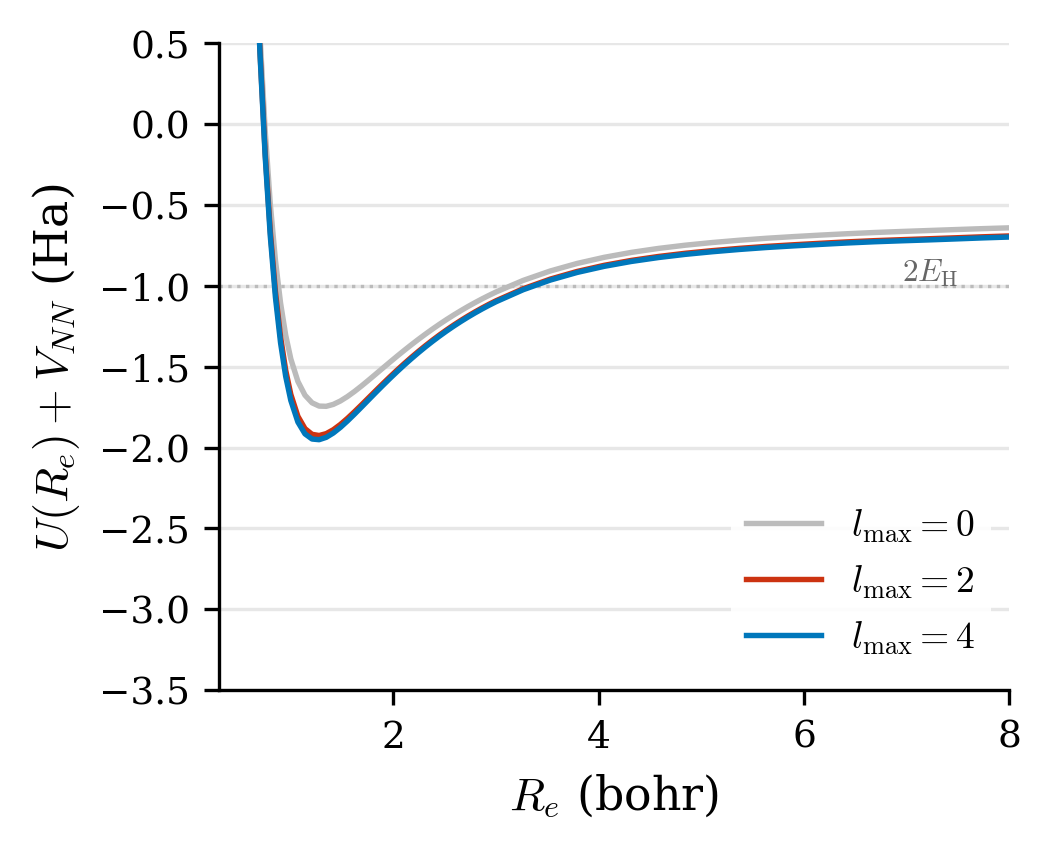
\includegraphics[width=\columnwidth]{paper_15_figures/adiabatic_potential.png}
\caption{Adiabatic potential $U(R_e) + V_{NN}$ at $R = 1.4$~bohr for
  $l_{\max} = 0$ (gray), 2 (red), and 4 (blue).  The well deepens with
  increasing $l_{\max}$ as quadrupolar and higher nuclear coupling channels
  open.  The dotted line marks the dissociation threshold $2E_{\rm H} = -1$~Ha.}
\label{fig:adiabatic}
\end{figure}

\subsection{The role of \texorpdfstring{$\pi$}{pi} channels}

The $\sigma$-only expansion ($m_{\max}=0$) uses Legendre polynomials
and has no $\Phi$-dependence.  Adding $\pi$~channels
($m_1 = \pm 1$, $m_2 = \mp 1$) introduces azimuthal flexibility
and consistently improves $D_e$ by ${\sim}7$~percentage points
at each $l_{\max}$ (Table~\ref{tab:convergence}).
This improvement is essential: at $l_{\max}=4$, the $\sigma$-only
result (87.0\%) falls below Paper~12's 92.4\%, while the
$\sigma{+}\pi$ result (94.1\%) exceeds it.

The $\pi$-channel coupling to $\sigma$ channels arises exclusively
through the $e$--$e$ multipole expansion (the nuclear potential is
diagonal in $m$ by axial symmetry).  The selection rule is
$q = m_1' - m_1 = -(m_2' - m_2)$, enforced by Wigner 3-$j$ symbols
in the coupling integrals.

\subsection{The remaining 5.9\% gap}

The gap between 94.1\% and exact has two sources:
\begin{enumerate}
  \item \textbf{Higher partial waves.}  The convergence from
    $l_{\max}=3$ (87.1\%) to $l_{\max}=4$ (94.1\%) with
    $\sigma{+}\pi$ channels suggests that $l_{\max} = 5$--$6$
    would recover further.
  \item \textbf{Higher $m$ channels.}  Within the adiabatic framework,
    $\delta$~channels ($m_{\max}=2$) add only ${\sim}0.3$~percentage
    points beyond $\pi$, indicating rapid convergence in $m_{\max}$.
    The 2D solver at higher $m_{\max}$ has not been tested.
\end{enumerate}

\subsection{Adiabatic vs.\ variational}

The adiabatic approximation overestimates $D_e$ by a remarkably
constant ${\sim}11\%$ across all channel counts
(Table~\ref{tab:convergence}).  This reflects the kinetic energy cost
of angular wavefunction variation with $R_e$: the non-adiabatic
coupling $P_{\nu\mu}(R_e) =
\braket{\Phi_\nu|\partial_{R_e}|\Phi_\mu}$ generates off-diagonal
terms in the radial kinetic energy that the adiabatic solver ignores.
At moderate channel counts ($N_{\rm ch} \le 13$), the overcounting is
masked by the larger basis truncation error.  At $N_{\rm ch} = 29$
($l_{\max}=4$, $m_{\max}=1$), the adiabatic result exceeds
$D_e^{\rm exact}$---a variational violation that signals the
breakdown of the single-channel approximation.
The 2D solver (Sec.~\ref{sec:2d_solver}) resolves this by treating
$R_e$ and the angular coordinates on equal footing.

\subsection{Double-adiabatic coupled-channel structure}

The Level~4 geometry has a double-adiabatic coupled-channel structure,
extending the single-adiabatic expansion of Paper~13:

\medskip
\noindent
\begin{tabular}{ll}
\textbf{Outer (nuclear):} & Slow variable $= R$;
  fast $=$ electronic problem \\
\textbf{Inner (electronic):} & Slow variable $= R_e$;
  fast $=$ angular channels \\
\textbf{Coupling:} & $P_{\nu\mu}(R_e) =
  \braket{\Phi_\nu|\partial_{R_e}|\Phi_\mu}$
\end{tabular}

\medskip
\noindent
The non-adiabatic coupling $P_{\nu\mu}$ encodes how the angular
channel functions change as $R_e$ varies.  Since the angular problem
depends on $R_e$ only through $\rho$, this coupling can be computed
as $P_{\nu\mu} = -(R/2R_e^2)\braket{\Phi_\nu|\partial_\rho|\Phi_\mu}$
via the Hellmann--Feynman theorem.

\paragraph{Fiber bundle interpretation.}
Mathematically, each adiabatic layer has the structure of a fiber
bundle: the slow variable is the base space, the channel Hilbert
space is the fiber, and $P_{\nu\mu}$ is the Berry connection.  The
Level~4 geometry thus realizes a double fiber bundle (outer: nuclear
base, electronic fiber; inner: hyperradial base, angular fiber).
However, the computation uses only coupled-channel methods---no
connection forms or holonomy calculations are required.

\subsection{Comparison with the He hierarchy}

The He hierarchy (Paper~13) has a single adiabatic layer: hyperradius
as slow variable, angular coordinates as fast.  The charge function
$C(\alpha,\theta_{12})$ is purely angular, so the angular eigenvalue
problem at fixed $R_e$ is a standard eigenvalue problem with no
parametric dependence.

In H$_2$, the molecular charge function depends on $\rho$, introducing
parametric variation of the angular problem.  This is structurally
analogous to the Born--Oppenheimer approximation in molecular physics:
nuclear coordinates $R$ play the role of slow parameters for the
electronic problem, while $R_e$ plays the same role within the
electronic problem itself.

\subsection{Heteronuclear systems and the charge-center origin}

The HeH$^+$ results demonstrate that the Level~4 framework
generalizes naturally to heteronuclear diatomics.  The key
structural change is the loss of inversion symmetry, which doubles
the channel count and activates odd-$k$ multipole coupling.

The charge-center origin (Eq.~\ref{eq:charge_center}) is not merely
a computational convenience but reflects a physical asymmetry: the
electronic wavefunction is concentrated around the heavier nucleus,
and placing the coordinate center there reduces the angular momentum
content needed to describe the lighter-nucleus contribution.
The improvement---approximately one unit of $l_{\max}$---is
consistent across channel counts and suggests that the charge
center is the natural expansion point for asymmetric Coulomb
problems in hyperspherical coordinates.

The 93.1\% recovery for HeH$^+$ at $l_{\max} = 4$ matches the
94.1\% achieved for H$_2$ at the same truncation, indicating
that the partial-wave expansion converges at comparable rates
once the origin is optimally placed.  This parity supports the
interpretation that the remaining ${\sim}6\%$ gap is dominated
by higher partial waves rather than by the heteronuclear
asymmetry itself.

\paragraph{Heteronuclear convergence and the composed-geometry
boundary.}
For heteronuclear diatomics, the angular eigenvalue $\mu_0$
converges exponentially with $l_{\max}$ at fixed $(R, R_e)$,
with decay rate $\beta \approx 0.42$ per unit $l_{\max}$ for a
$6{:}1$ charge ratio at $\rho = 0.7$ (exponential fit
$R^2 = 0.997$).  At $l_{\max} = 10$, the eigenvalue is within
1\% of the Richardson-extrapolated limit.

The angular wavefunction spreading that necessitates high
$l_{\max}$ is entirely nuclear in origin: removing all
electron--electron off-diagonal coupling leaves
$w(0{,}0) = 0.9998$, while removing the nuclear coupling yields
$w(0{,}0) = 0.243$.  Thus the Level~4 solver itself converges
well for asymmetric bonds; the $R_{\rm eq}$ divergence reported
in Paper~17~\cite{paper17} is a property of the composed geometry
framework (specifically, the Phillips--Kleinman pseudopotential),
not of the Level~4 coordinate system.

While eigenvalue convergence at fixed geometry is exponential,
the \emph{equilibrium geometry} $R_{\rm eq}$ drifts linearly
with $l_{\max}$ in the adiabatic solver: $+0.262$~bohr per
$l_{\max}$ for bare HeH$^+$ (no pseudopotential, no composition).
The mechanism is that asymmetric nuclear coupling populates odd-$l$
channels---forbidden in homonuclear systems---which preferentially
stabilize large-$R$ configurations.  H$_2$ places 94\% of its
channel weight in the $(0{,}0)$ channel, while HeH$^+$ places only
68\%, with 20\% in odd-$l$ channels.  This drift is an artifact
of the single-channel adiabatic approximation; the variational
2D solver (Sec.~\ref{sec:2d_solver}), which treats
$(R_e, \alpha)$ simultaneously, does not suffer from this
truncation and is the identified path to eliminating the
$l_{\max}$ divergence in composed geometries.

\subsection{Spectral Laguerre radial solver}
\label{sec:spectral_radial_l4}

Following the spectral Laguerre pattern established for Level~2
(Paper~11~\cite{loutey_paper11}) and Level~3
(Paper~13~\cite{loutey_paper13}), we replace the finite-difference
$R_e$ grid with a Laguerre spectral basis for all three Level~4
solution pathways: adiabatic, coupled-channel, and variational 2D.

The basis functions are identical to Eq.~(31) of
Paper~13~\cite{loutey_paper13}, with the substitution $R \to R_e$
and Dirichlet boundary condition enforced by a $(R_e - R_{e,\min})$
prefactor.  The overlap and kinetic matrices are computed algebraically
via three-term Laguerre recurrence (no quadrature), while the effective
potential $U_{\mathrm{eff}}(\rho)$ is evaluated by Gauss--Laguerre
quadrature at each angular sweep point~$\rho$.

Table~\ref{tab:spectral_l4_convergence} shows the convergence
behavior.  The optimal basis size is $n_{\mathrm{basis}} = 20$;
mild overlap matrix conditioning degradation appears at
$n_{\mathrm{basis}} \geq 25$.

\begin{table}[h]
\caption{Convergence of the spectral Laguerre radial solver for
Level~4 (H$_2$, $l_{\max} = 2$, $R = 1.4$~bohr).
FD reference ($N_R = 400$): $E = -1.87131$~Ha.}
\label{tab:spectral_l4_convergence}
\begin{ruledtabular}
\begin{tabular}{rd}
  $n_{\mathrm{basis}}$ & \multicolumn{1}{c}{$\Delta E_{\mathrm{FD}}$ (Ha)} \\
  \hline
  10 & 2.5 \times 10^{-5} \\
  15 & 7.5 \times 10^{-6} \\
  20 & 5.0 \times 10^{-6} \\
  25 & 4.8 \times 10^{-5} \\
  30 & 5.8 \times 10^{-5} \\
\end{tabular}
\end{ruledtabular}
\end{table}

The adiabatic pathway achieves a $16\times$ dimension reduction
($N_R = 400 \to n_{\mathrm{basis}} = 25$) with $< 0.0005$~Ha
agreement.  The 2D pathway achieves $5\times$ reduction.

A key structural finding is that the spectral substitution does
\emph{not} improve total wall time.  The angular eigenvalue sweep---
building $H_{\mathrm{ang}}$ at $\sim\!130$ $\rho$-values, each
requiring a full angular diagonalization---accounts for 99\% of
Level~4 runtime.  The FD radial solve uses \texttt{eigh\_tridiagonal}
($O(N)$, sub-ms), which is already optimal.  Accelerating Level~4
requires faster angular solves or caching strategies, not a faster
radial solver.

\subsection{Spectral Jacobi angular solver}
\label{sec:spectral_angular_l4}

Having identified the angular eigenvalue sweep as the 99\% bottleneck
(Sec.~\ref{sec:spectral_radial_l4}), we replace the finite-difference
angular solver with a spectral Jacobi polynomial basis.

The free angular Hamiltonian has exact eigenvalues given by the SO(6)
Casimir: $\nu(\nu+4)/2$ for angular momentum quantum number~$\nu$.
We use Jacobi polynomials as the spectral basis, with these Casimir
eigenvalues as the free spectrum.  The electron--electron coupling
matrix $V_{ee}$ is precomputed once via Gaunt-type angular integrals
(independent of~$\rho$), while the nuclear coupling $V_{\rm nuc}$
scales linearly with~$\rho$.  At each sweep point, the full angular
Hamiltonian is assembled as
\begin{equation}
  H_{\rm ang}(\rho) = H_{\rm free} + \rho \, V_{\rm nuc} + V_{ee}
\end{equation}
and diagonalized.

Table~\ref{tab:spectral_angular_l4} compares the finite-difference
and spectral angular solvers.

\begin{table}[h]
\caption{Finite-difference vs.\ spectral Jacobi angular solver for
Level~4 (H$_2$, $l_{\max} = 2$, 130 $\rho$-points).}
\label{tab:spectral_angular_l4}
\begin{ruledtabular}
\begin{tabular}{lcc}
  Metric & FD ($n_\alpha = 200$) & Spectral ($n_{\rm basis} = 10$) \\
  \hline
  Matrix dimension      & ${\sim}1000$ & 50 \\
  Angular sweep time    & 39.9~s       & 0.15~s \\
  $U_{\min}$ difference & ---          & $< 2 \times 10^{-5}$~Ha \\
  $D_e$ (\% exact)      & 90.0\%       & 89.7\% \\
\end{tabular}
\end{ruledtabular}
\end{table}

The spectral basis achieves a $20\times$ dimension reduction
($1000 \to 50$) and a $269\times$ speedup on the angular sweep
(39.9~s $\to$ 0.15~s for 130 $\rho$-points).  The $U_{\min}$
agreement is $< 2 \times 10^{-5}$~Ha.  The 0.3\% $D_e$ shift
(90.0\% $\to$ 89.7\%) reflects removal of finite-difference error
cancellation, not a regression.

Combined with the spectral Laguerre radial solver
(Sec.~\ref{sec:spectral_radial_l4}), the angular sweep fraction
drops from 99\% to approximately 50\% of total Level~4 runtime.
The angular eigenvalues $\mu(\rho)$ remain transcendental---computed
by diagonalization at each $\rho$-point---but the per-point cost
is now a $50 \times 50$ eigensolve rather than
$1000 \times 1000$.

The default solver remains \texttt{angular\_method='fd'};
the spectral variant is accessed via
\texttt{angular\_method='spectral'}.

%% ========================================================================
%% VIII. CONCLUSION
%% ========================================================================
\section{Conclusion}
\label{sec:conclusion}

We have introduced the Level~4 natural geometry for two-center,
two-electron molecules: molecule-frame hyperspherical coordinates
$(R_e,\alpha,\theta_1,\theta_2,\Phi)$ parameterized by
$\rho = R/(2R_e)$.

The main results are:
\begin{enumerate}
  \item The electron--electron cusp at $\alpha = \pi/4$,
    $\theta_{12} = 0$ is $R$-independent, resolving it as a boundary
    condition for all molecular geometries.
  \item The angular eigenvalue problem depends on $(R,R_e)$ only through
    $\rho$, collapsing a 2D parameter sweep to 1D.
  \item The gerade--quadrupole constraint explains the dramatic jump at
    $l_{\max}=2$ (31\% $\to$ 80\%): the first nuclear coupling from
    the $(0,0)$ channel requires $\Delta l = 2$.
  \item $\pi$-orbital channels ($m \ne 0$) are essential, providing
    ${\sim}7$~percentage points of improvement at each $l_{\max}$.
    Without $\pi$ channels, Level~4 ($\sigma$-only, 87.0\%) falls
    below Paper~12 (92.4\%); with them, it exceeds it (94.1\%).
  \item A variational 2D solver avoids the ${\sim}11\%$ systematic
    overestimate of the adiabatic approximation, giving rigorous
    bounds.
  \item The framework extends to heteronuclear diatomics (HeH$^+$)
    by removing the gerade constraint, activating odd-$k$ multipole
    coupling, and shifting the origin to the charge center
    (Eq.~\ref{eq:charge_center}), recovering 93.1\% of the exact
    $D_e$ at $l_{\max} = 4$ with $\sigma{+}\pi$ channels.
\end{enumerate}

The natural geometry hierarchy is now:
\begin{center}
\begin{tabular}{clll}
\toprule
Level & System & Geometry & Best $D_e$ \\
\midrule
1 & H       & $S^3$ (Fock)        & $<0.1\%$ error \\
2 & H$_2^+$ & Prolate spheroid    & 0.70\% error \\
3 & He      & Hyperspherical      & 0.05\% error \\
4 & H$_2$   & Mol.-frame hypersp. & 94.1\% \\
4 & HeH$^+$ & Mol.-frame hypersp. & 93.1\% \\
\bottomrule
\end{tabular}
\end{center}

Future work includes: (i)~$l_{\max} \ge 5$ with $\sigma{+}\pi$ channels
in the 2D solver; (ii)~non-uniform or finite-element radial grids
for improved 2D convergence; (iii)~full potential energy surfaces
with nuclear dynamics.

\paragraph{The locked-core boundary.}
Extension to systems with core electrons (e.g., LiH) presents a
fundamental challenge.  The locked-shell approach---treating core
electrons as a fixed Hartree potential while solving the active electrons
in molecular coordinates---violates the discrete lattice principle of
Paper~0 by converting core electrons from graph nodes to a continuous
potential.  This architectural mismatch produces systematic errors: the
equilibrium geometry is too short ($R_{\rm eq} \approx 2.5$~bohr vs.\
experimental 3.015~bohr) regardless of how the core potential is modeled
(bare $Z_{\rm eff}$, Clementi--Raimondi screening, or Hartree with
penetration).

The resolution likely requires either (a)~a full 4-electron Level~4
treatment with no locked core, which would involve an 8-dimensional
angular eigenvalue problem, or (b)~identification of the natural graph
structure that connects atomic core geometry ($S^3$) to molecular valence
geometry (hyperspherical), preserving discrete topology throughout.
HeH$^+$ succeeds because it has no core electrons; the two active
electrons live entirely in the molecular geometry.

%% ========================================================================
%% REFERENCES
%% ========================================================================
\begin{thebibliography}{20}

\bibitem{fock1935}
V.~A.~Fock,
``Zur Theorie des Wasserstoffatoms,''
Z.~Phys.\ \textbf{98}, 145 (1935).

\bibitem{lin1995}
C.~D.~Lin,
``Hyperspherical coordinate approach to atomic and other
Coulombic three-body systems,''
Phys.\ Rep.\ \textbf{257}, 1 (1995).

\bibitem{macek1968}
J.~Macek,
``Properties of autoionizing states of He,''
J.~Phys.\ B \textbf{1}, 831 (1968).

\bibitem{kolos1968}
W.~Kolos and L.~Wolniewicz,
``Improved theoretical ground-state energy of the hydrogen molecule,''
J.~Chem.\ Phys.\ \textbf{49}, 404 (1968).

\bibitem{james1933}
H.~M.~James and A.~S.~Coolidge,
``The ground state of the hydrogen molecule,''
J.~Chem.\ Phys.\ \textbf{1}, 825 (1933).

\bibitem{morse1953}
P.~M.~Morse and H.~Feshbach,
\emph{Methods of Theoretical Physics}
(McGraw-Hill, New York, 1953), Chap.~10.

\bibitem{paper7}
J.~Loutey,
``The Dimensionless Vacuum: Scale-Invariant Graph Topology
and the Schr\"odinger Equation'' (Paper~7 in the Geometric Vacuum series).

\bibitem{paper11}
J.~Loutey,
``Molecular Fock Projection: Prolate Spheroidal Lattice
for Diatomic Molecules'' (Paper~11 in the Geometric Vacuum series).

\bibitem{paper12}
J.~Loutey,
``Algebraic Two-Electron Integrals: Neumann Expansion
for $V_{ee}$ on the Prolate Spheroidal Lattice''
(Paper~12 in the Geometric Vacuum series).

\bibitem{paper13}
J.~Loutey,
``Hyperspherical Lattice: Two-Electron Atoms as
Coupled-Channel Graphs'' (Paper~13 in the Geometric Vacuum series).

\bibitem{paper17}
J.~Loutey,
``Composed Natural Geometries for Core-Valence Diatomics:
LiH and BeH$^+$ from Discrete Graph Topology''
(Paper~17 in the Geometric Vacuum series).

\bibitem{bishop1977}
D.~M.~Bishop and L.~M.~Cheung,
``A theoretical investigation of HeH$^+$,''
J.~Mol.\ Spectrosc.\ \textbf{75}, 462 (1979).

\end{thebibliography}

\end{document}
